% \documentclass[pdftex,12pt,a4paper]{report}
\documentclass[12pt,a4paper]{article}

\usepackage{anysize}
\marginsize{3cm}{3cm}{3cm}{3cm}
\usepackage{graphicx}
\usepackage{t1enc}
\usepackage[MeX]{polski}
\usepackage[utf-8]{inputenc}
\usepackage[T1]{fontenc}
\usepackage{subfigure}

\usepackage{fancyhdr}
\setlength{\headheight}{15pt}
\pagestyle{fancy}

\newcommand{\HRule}{\rule{\linewidth}{0.5mm}}

\begin{document}

\begin{titlepage}

\begin{center}

% Upper part of the page

\includegraphics[width=0.15\textwidth]{./img/logo.eps}\\[1cm]

\textsc{\LARGE Akademia Górniczo-Hutnicza}\\[1.5cm]

\textsc{\Large Bazy Danych}\\[0.5cm]


% Title 
\HRule \\[0.4cm]
{ \huge \bfseries Rozkład Jazdy}\\[0.4cm]

\HRule \\[1.5cm]

% Author and supervisor
\begin{minipage}{0.4\textwidth}
\begin{flushleft} \large
\emph{Autorzy:}\\
Tomasz \textsc{Huczek}\\
Andrzej \textsc{Jasiński}
\end{flushleft}
\end{minipage}
\begin{minipage}{0.4\textwidth}
\begin{flushright} \large
\emph{Konsultant:} \\
Dr inż. \textsc{Antoni Ligęza}
\end{flushright}
\end{minipage}

\vfill

% Bottom of the page
{\large \today}

\end{center}

\end{titlepage}


\fancyhf{}

\lhead{Tomasz Huczek, Andrzej Jasiński}
\rhead{\today}
\rfoot{\thepage}

\begin{abstract}
 Projekt konceptualny zawierający kolejne etapy projektowania i realizacji aplikacji bazy danych.
\end{abstract}


\tableofcontents
\newpage


\section{Sformułowanie zadania projektowego}

\textit{Podanie przedmiotu projektowania, jego celów,
przeglądu zadań, specyfiki i uwarunkowań.} \\

Przedmiotem projektowania jest stworzenie bazy danych oraz interfejsu użytkownika służacego do przechowywania informacji oraz do wyświetlania i zarządzania rozkładami jazdy. Rozkłady jazdy dotyczą pojazdów komunikacji miejskiej takich jak autobusy i tramwaje.
Aplikacja ma za zadanie w sposób prosty oraz intuicyjny służyć użytkownikowi, wyświetlając rozkłady jazdy w różnych postaciach zależnie od wymagań użytkownika. Dodatkowo aplikacja dysponuje możliwością wyszukiwania połączeń pomiędzy przystankami\footnote{Wyszukiwanie połączeń jest ograniczone do połączeń składających się maksymalnie z dwóch lini}.

Projekt będzie zbudowany w oparciu o bazę PostgreSQL, natomiast interfejs użytkownika stworzony zostanie w technologi XHTML w połączeniu z PHP.

\section{Analiza stanu wyjściowego}


%\textit{Analiza stanu zastanego, uwarunkowań prawnych, przyjętego
%obiegu istniejącej dokumentacji, analiza istniejącego systemu elektronicznego
%przetwarzania danych (aktualnej bazy), analiza występujących problemów, etc. pomocne
%mogą być scenariusze postępowania i ich analiza (elementy, obiekty, charakterystyki,
%atrybuty, struktura, przepływ danych, powiązania, relacje, ograniczenia funkcjonalności).} \\
Nasz system budujemy od podstaw, więc nie mamy żadnego istniejącego systemu badź dokumentacji. Oczywiście istnieją podobne rozwiązania,
jak np. strona krakowskiego MPK i chcemy osiągnąć podobną funkcjonalność. Niestety, z powodu braku wystarczającej czasu oraz pewnych ograniczeń nie możemy na tym etapie wykonać pełnej implementacji wyszukiwarki połączeń.



\section{Analiza wymagań użytkownika}

\textit{Na tym etapie należy określić podstawowe
cele, zadania i funkcjonalność jakie mają być realizowane przez projektowaną bazę danych
oraz ew. wymagania dotyczące projektu i dokumentacji. Dobrze byłoby, aby użytkownik
na bieżąco współuczestniczył w projektowaniu i implementacji oraz wnosił swoje uwagi.
Należy zidentyfikować wymagania jawne i niejawne.} \\


\section{Określenie scenariuszy użycia}
\textit{Scenariusze użycia pozwolą na konstrukcję diagramów
DFD i STD oraz hierarchii funkcji.}
W projekcie przewidujemy dwa główne scenariusze użytkowania : użytkownik i administrator.\\
Użytkownik będzie mógł:
\begin{list}{*}{}
\item poszukiwać połączeń, przystanków, linii oraz przystanków w pobliży zadanej ulicy
\item wyświetlać wybrany rozkład jazdy
\end{list}

Administrator będzie odpowiedzialny za dodawanie, edycję oraz usuwanie danych z rozkładu tzn:
\begin{list}{*}{}
\item dodawać nowe przystanki, edytować i usuwać już istniejące
\item dodawać linie, przystanek po przystanku i określać czas podróży pomiędzy przystankami,
\item usuwać linie,
\item usuwać przystanki, pod warunkiem że przez wybrany do usunięcia przystanek nie przebiega trasa żadnej z linii,
\item modyfikować istniejące trasy oraz generować i modyfikować rozkłady jazdy
\end{list}



\section{Identyfikacja funkcji}
Określenie podstawowych funkcji realizowanych w bazie danych.
\section{Analiza hierarchii funkcji projektowanej aplikacji (FHD - Functional Hierarchy
Diagram)}
\textit{Określenie struktury zależności hierarchicznych pomiędzy jednostkami
analizowanego systemu, zwłaszcza w zakresie specyfikacji wymagań funkcjonalnych.
Specyfikacja funkcji (funkcjonalności) projektowanego systemu.} \\

\begin{enumerate}
    \item Funkcje administratora
    \begin{enumerate}
        \item Zarządzanie liniami
                \begin{enumerate}
                    \item Dodawanie linii
                    \item Usuwanie linii
                    \item Edycja linii
                \end{enumerate}
        \item Zarządzanie przystankami
                \begin{enumerate}
                    \item Dodawanie nowego przystanku
                    \item Edycja istniejącego przystanku
                    \item Usuwanie przystanku
                \end{enumerate}
    \end{enumerate}

    \item Funkcje użytkownika
     \begin{enumerate}
        \item Przeszukiwanie bazy
            \begin{enumerate}
                \item Poszukiwanie możliwych połączeń pomiędzy dwoma przystankami
                \item Przeglądanie dostepnych linii
                \item Poszukiwanie przystanku według nazwy
                \item Poszukiwanie przystanku według nazwy ulicy
                \item Wyświetlenie rozkładu jazdy dla danej linii dla danego przystanku
            \end{enumerate}

     \end{enumerate}

\end{enumerate}





\section{Budowa i analiza diagramu przepływu danych - Data Flow Diagram }
\textit{Ma na celu określenie przepływu danych (wejścia, wyjścia, operacje, przechowywanie) oraz
elementów sterowania tym przepływem, co może być pomocne dla tworzenia aplikacji.
Specyfikacja danych wejściowych i wyjściowych.}

\section{Wybór encji (obiektów) i ich atrybutów}

Podstawowymi encjami w naszym projekcie są \textbf{Linia} oraz \textbf{Przystanek}. 
Ich atrybuty opisują fizyczne odpoiwedniki, przechowując takie informacje jak \textit{numer}
lini, jej \textit{typ} oraz \textit{opis} słowny. Przystanek jest opisnay przez atrybut: 
\textit{nazwa} oraz \textit{ulica} - nazwa ulicy przy jakiej dany przystanek się znajduje.
Są to obiekty reprezentujące fizyczne linie autobusowe poruszające się po kolejnych 
obiektach jakimi są przystanki. Kolejnymi encjami są \textbf{Trasy}, które wiążą 
daną linię z listą przystanków. Obiektami reprezentującymi godziny odjazdów autobusów
z kolejnych przystanków są odpowiednio \textbf{Odjazdy} oraz \textbf{Przesuniecia}.
Pierwszy obiekt przechowuje informacje o godzinach odjazdów autobusów z pętli, i jest 
przypisany do danej lini. Odjazdy posiadają atrybuty \textit{kierunek} oraz \textit{godzina}.
\textbf{Przesuniecia} określają przesunięcia czasowe (atrybut \textit{offset}) na przystankach 
względem pętli i są przyporządkowane do lini oraz przystanku (według wpisu z tabeli \textit{trasy}.

\section{Projektowanie powiązań (relacji) pomiędzy encjami}

% \textit{Konstrukcja diagramu ERD
% (Entity-Relationship Diagram); jest to zasadniczy etap procesu projektowania struktury
% bazy danych. Identyfikacja klas encji, ich atrybutów, zdefiniowanie (określenie) kluczy.
% Tablica krzyżowa powiązań, eliminacja powiązań wiele-do-wielu. Konstrukcja diagramu
% ERD.} \\

Diagram ERD przedstawiono na rysunku \ref{fig:erd}.

\begin{figure}[!htp]
    \centering
    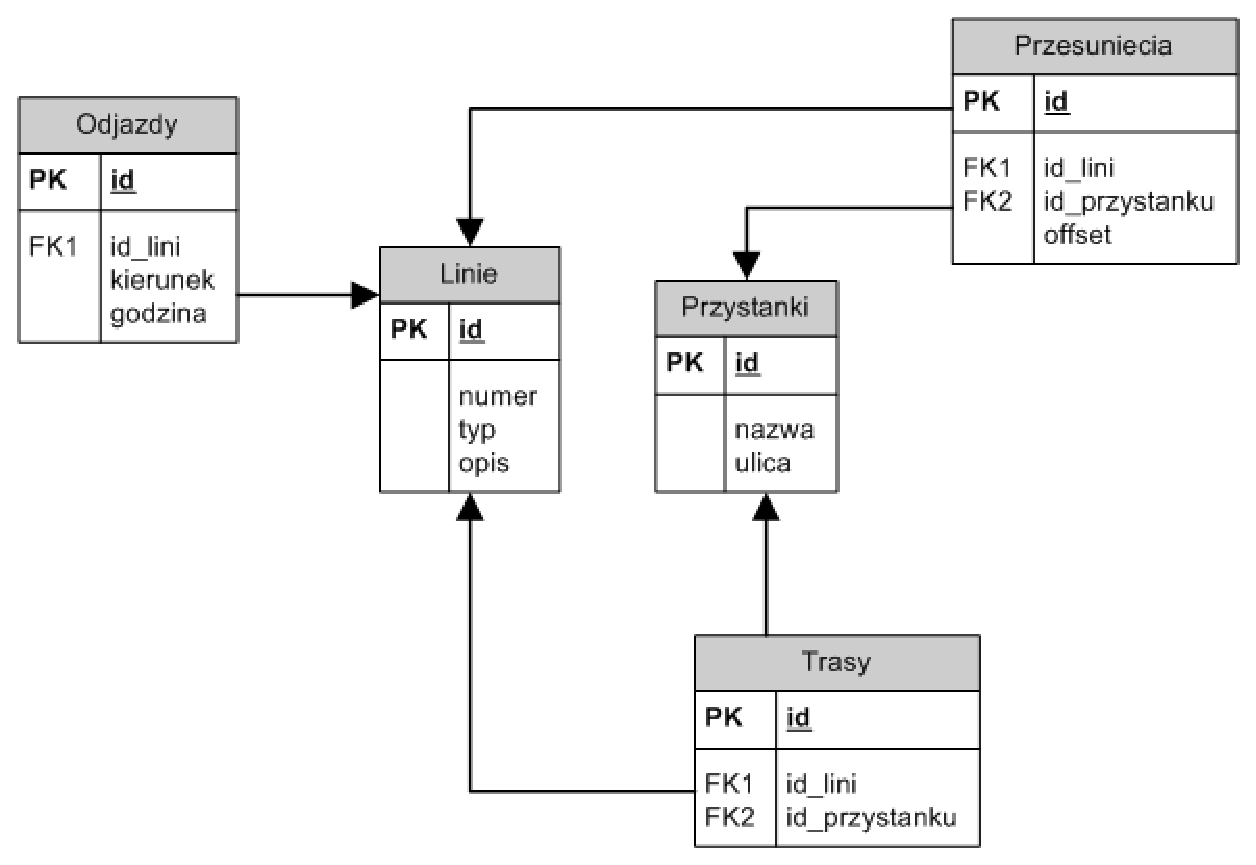
\includegraphics[width=0.8\textwidth]{./img/bus-agenda-erd.eps}
    \caption{Diagram ERD}
    \label{fig:erd}
\end{figure}


\section{Projekt diagramów STD (State Transition Diagram - diagramy przejść pomiędzy
stanami)}

% \textit{Wykonanie w oparciu o scenariusze użycia i strukturę bazy danych. Pomocny do
% budowy interfejsu aplikacji.} \\
\begin{figure}[!htp]
  \centering
  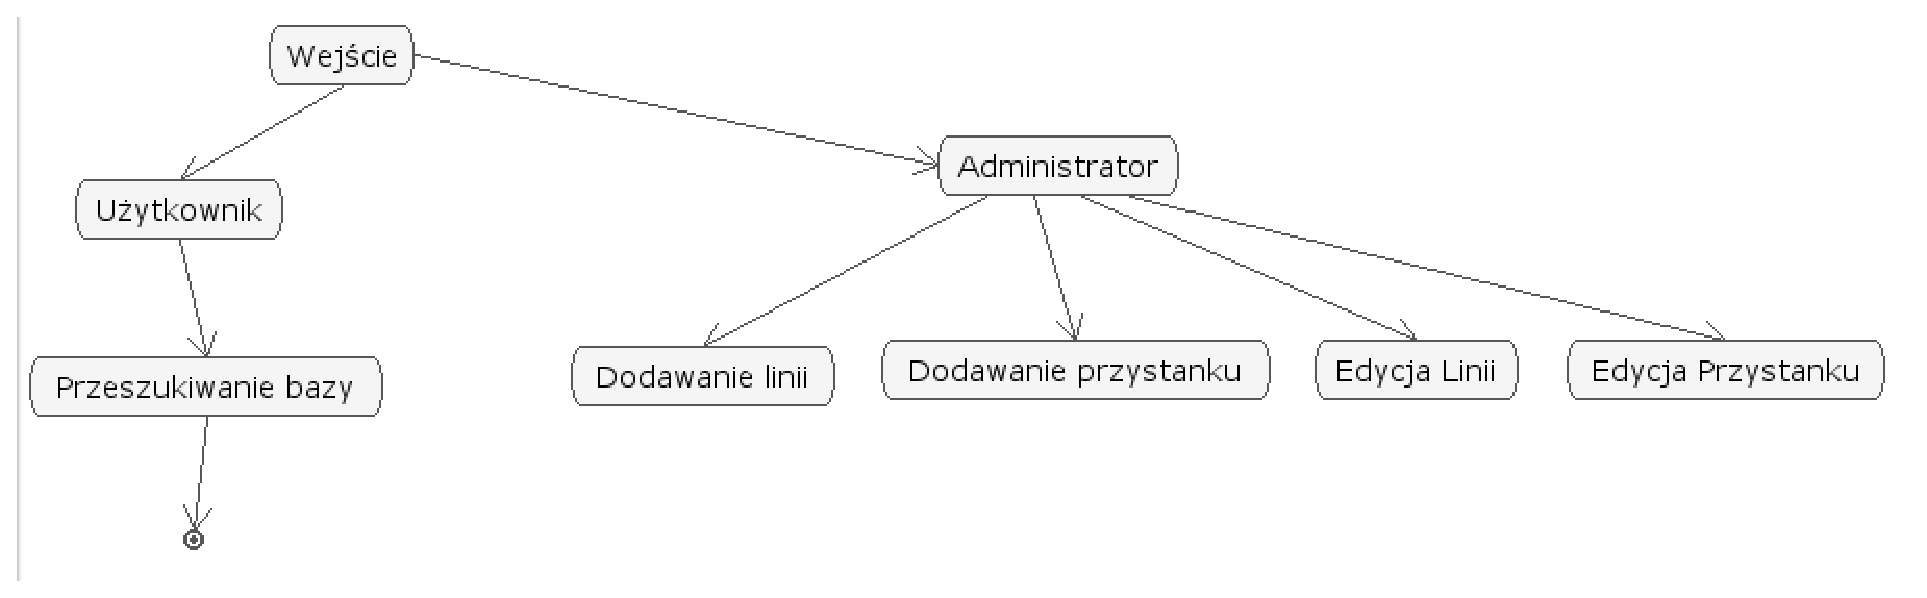
\includegraphics[width=0.8\textwidth]{./img/state.eps}
  \caption{Diagram STD}
  \label{fig:scr3}
\end{figure}


\clearpage
\addcontentsline{toc}{section}{Literatura}
\begin{thebibliography}{99}
\bibitem{bib:onelecture} Jakaś książka
\end{thebibliography}

\end{document}
